\documentclass{article}
\usepackage[utf8]{inputenc}
\usepackage[utf8]{vietnam}
\usepackage[left=4cm,right=4cm]{geometry}
\usepackage{indentfirst}
\usepackage{graphicx}
\usepackage{minted}
\usepackage{fancyvrb}
\usepackage{url}
\usepackage{hyperref}
\usepackage{fontawesome5}
\usepackage{tikz}
\usetikzlibrary{backgrounds}
\usetikzlibrary{shapes.misc}
\usetikzlibrary{arrows.meta}
\usetikzlibrary{fit}
\usetikzlibrary{positioning}
\usetikzlibrary{calc}

\hypersetup{colorlinks=true,urlcolor=red,unicode=true}

\title{\textbf{Bài tập cuối khóa Cloud Computing tại Viettel Network}}
\author{Ngô Quang Dương -- 17020191 \\ K62, UET -- VNU}
\date{\today}

\begin{document}

\maketitle

\begin{abstract}
Trong báo cáo ngắn này, em sẽ trình bày quá trình chuẩn bị, cấu hình và ý tưởng của em để đạt được kết quả cho bài tập cuối khóa. Báo cáo được gửi kèm các file inventory, playbook, \ldots
\end{abstract}


\tableofcontents

\newpage

\section{Chuẩn bị}

\par Ý tưởng của em là sử dụng \textbf{AWS EC2} để tạo hai máy ảo làm \textit{managed nodes}. Thông qua \textbf{Ansible}, em sẽ cài đặt \textbf{Docker} và các \textit{images} lên hai máy đó.
https://www.youtube.com/watch?v=2BPx4nPgPgw
\par Quá trình chạy \textit{playbook} được ghi lại trong \href{https://www.youtube.com/watch?v=2BPx4nPgPgw}{\underline{YouTube}} (lưu ý cần bật subtitle).

\par Mã nguồn của bài tập được lưu tại \href{https://github.com/duong755/vtnet-course}{\underline{GitHub}}.

\subsection{Tạo 2 máy ảo với AWS EC2}

\begin{figure}[htp]
    \centering
    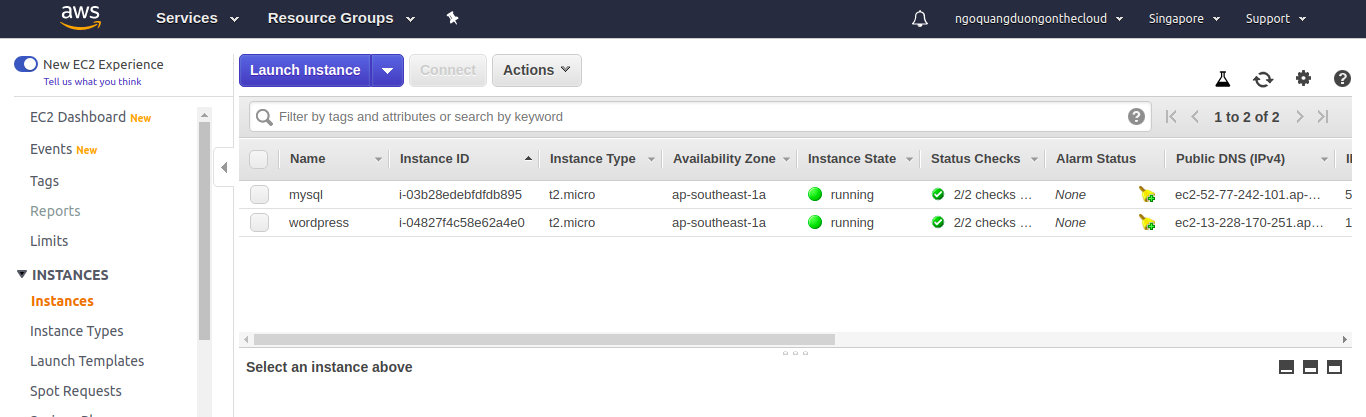
\includegraphics[width=\textwidth]{ec2.png}
    \caption{Hai máy ảo EC2}
\end{figure}

\par Thông tin chi tiết hơn về 2 máy này:

\begin{itemize}
    \item Máy 1
    \begin{itemize}
        \item Tên: mysql
        \item Username mặc định: ubuntu
        \item Chạy trên Ubuntu 18.04
        \item Dùng để cài mysql image
        \item Cho phép kết nối vào cổng 22 (SSH) và 3306 (MYSQL)
    \end{itemize}
    \item Máy 2
    \begin{itemize}
        \item Tên: wordpress
        \item Username mặc định: ubuntu
        \item Chạy trên Ubuntu 18.04
        \item Dùng để cài wordpress image
        \item Cho phép kết nối vào cổng 22 (SSH) và 80 (HTTP)
    \end{itemize}
\end{itemize}

\subsection{Key pairs và SSH config}

\par \textbf{AWS EC2} cho phép kết nối đến các máy ảo thông qua \textbf{SSH}. Trước khi các máy ảo được khởi tạo, \textbf{AWS EC2} tạo ra một file \texttt{.pem} -- cần tải file này về, đặt vào thư mục \texttt{\textasciitilde/.ssh/}.

\par Để cho đơn giản, cả hai máy trên dùng chung một file \texttt{.pem}

\par SSH config có nội dung như sau

\begin{Verbatim}[frame=single]
Host mysql
    HostName public_ip_of_mysql_instance
    User ubuntu
    Port 22
    IdentitiesOnly yes
    IdentityFile path/to/pem

Host wordpress
    HostName public_ip_of_wordpress_instance
    User ubuntu
    Port 22
    IdentitiesOnly yes
    IdentityFile path/to/pem
\end{Verbatim}

\par File sshconfig tuy không được sử dụng bởi \textbf{Ansible} nhưng cần thiết để lệnh kết nối được viết ra nhanh chóng.

\section{Nội dung chính}

\par GitHub repo không lưu file inventory.

\par Inventory được tạo ra từ file \texttt{inventory\_generator.py} (do public IP của máy ảo không cố định)

\subsection{File inventory}
\begin{minted}[frame=single]{ini}
[homework]

[mysql]
public_ip_of_mysql_instance

[wordpress]
public_ip_of_wordpress_instance

[homework:children]
mysql
wordpress

[homework:vars]
ansible_python_interpreter=/usr/bin/python
ansible_ssh_user=ubuntu
ansible_ssh_private_key_file=~/.ssh/homework.pem
\end{minted}

\par Trong đó, \texttt{homework} là group chứa cả hai \textit{managed nodes}.

\par Hai \textit{managed nodes} được truy cập đến qua \textbf{SSH} với file key được chỉ định trong biến \texttt{ansible\_ssh\_private\_key\_file}.

\par \texttt{homework} chứa hai group con \texttt{mysql}, \texttt{wordpress}. Mỗi group này lần lượt gồm host của \textit{managed nodes}  được dùng để cài đặt \textbf{MySQL} và \textbf{Wordpress} image. IP được cung cấp trong hai group này là public IP v4 của hai máy ảo.

\par Mục đích của việc tạo group con là để IP được cô lập trong file \textit{inventory} và khi sử dụng \textit{playbook} thì chỉ cần đến tên group chứa IP đó.

\subsection{Playbook tasks}

\par File playbook là \texttt{homework.yaml}

\par Việc cài đặt \textbf{Docker} được chia làm các tasks sau (thực hiện trên cả 2 nodes):

\begin{itemize}
    \item Cài các packages: \texttt{apt-transport-https}, \texttt{ca-certificates}, \texttt{curl}, \texttt{gnupg-agent}, \texttt{software-properties-common}
    \item Thêm GPG key của \textbf{Docker}
    \item Thêm \textbf{Docker} repository
    \item \texttt{apt update}
    \item \texttt{dpkg --configure -a}
    \item \texttt{apt upgrade}
    \item Cài các packages: \texttt{docker-ce}, \texttt{docker-ce-cli}, \texttt{containerd.io}
    \item Tạo group docker
    \item Thêm user ubuntu và group docker
    \item Khởi động lại cả 2 nodes
\end{itemize}

\par Sau khi các tasks chung trên hoàn tất, \textit{playbook} thực hiện các task riêng cho từng node. Cụ thể là pull image, sau đó chạy container.

\newpage
\subsection{Mô hình lab}

\begin{figure}[htpb]
    \centering
    \begin{tikzpicture}[>={Stealth[round]}]
        \tikzset{framednode/.style={rounded corners,draw=black}}

        \node (aws) {AWS EC2};

        \node [at={($(aws.south west) + (-2.5cm,-1.5cm)$)}] (node 1) {
            \begin{tikzpicture}
                \node (mysql) {\underline{Managed Node}};
                \begin{scope}[shift={($(mysql.south) + (0cm,-0.4cm)$)}]
                    \node (mysql container name) {\faDocker{}\ MySQL Container};
                    \node [below=0.1cm of mysql container name,align=center] (mysql port) { SSH: 22, MySQL: 3306 };
                \end{scope}

                \begin{scope}[on background layer]
                    \node (mysql container) [framednode,fill=blue!20,draw=blue,fit=(mysql container name)(mysql port)] {};
                \end{scope}

                \begin{scope}[on background layer]
                    \node (mysql node) [framednode,fit=(mysql container)(mysql)] {};
                \end{scope}
            \end{tikzpicture}
        };

        \node [at={($(aws.south east) + (2.5cm,-1.5cm)$)}] (node 2) {
            \begin{tikzpicture}
                \node (wordpress) {\underline{Managed Node}};
                \begin{scope}[shift={($(wordpress.south) + (0cm,-0.4cm)$)}]
                    \node (wordpress container name) {\faDocker{}\ WordPress Container};
                    \node [below=0.1cm of wordpress container name,align=center] (wordpress port) { SSH: 22, HTTP: 80 };
                \end{scope}

                \begin{scope}[on background layer]
                    \node (wordpress container) [framednode,fill=cyan!30,draw=cyan,fit=(wordpress container name)(wordpress port)] {};
                \end{scope}

                \begin{scope}[on background layer]
                    \node (wordpress node) [framednode,fit=(wordpress container)(wordpress)] {};
                \end{scope}
            \end{tikzpicture}
        };

        \draw[<-] (node 1) -- (node 2) node[midway,above,align=center,text width=2cm] {Database Connection};

        \begin{scope}[on background layer]
            \node (ec2) [framednode,fit=(node 1)(node 2)(aws)] {};
        \end{scope}

        \node[at={($(ec2.south) + (0cm,-2cm)$)}] (control node name) {\underline{Control Node}};
        \node[below=0.1cm of control node name,text width=4cm] (control node components) {
            {\vbox{\begin{list}{--}{\itemsep=0pt\topsep=0pt\leftmargin=10pt}
                \item Ansible
                \item Modules
                \item Playbook
                \item Inventory
                \item Vault Password File
            \end{list}}}
        };
        \begin{scope}[on background layer]
            \node (control node) [framednode,fit=(control node name)(control node components)] {};
        \end{scope}


        \path[->]
          (control node) edge[bend left=15] node[left] {SSH connection} (node 1)
          (control node) edge[bend right=15] node[right] {SSH connection} (node 2);
    \end{tikzpicture}
    \caption{Mô hình lab}
\end{figure}

\section{Bonus}

\subsection{Dynamic inventory}

\par Các máy ảo \textbf{EC2} có một đặc điểm là public IP sẽ được reset mỗi khi tắt đi -- bật lại (nhưng restart thì không). Điều này dẫn tới một điều bất tiện là phải copy paste public ip mới vào file inventory mỗi khi thực hiện việc tắt đi bật lại.

\par Để khắc phục điều này, em sử dụng \textbf{Python} và \textbf{AWS SDK} dành cho \textbf{Python} để tự động lấy public IP về. Em đã chuẩn bị:

\begin{itemize}
    \item Cài AWS SDK cho Python -- Boto3
    \item Thêm region của máy ảo vào file \texttt{\textasciitilde/.aws/config}
    \begin{minted}{ini}
    [default]
    region = ap-southeast-1
    \end{minted}
    \item Thêm access key id và access key secret vào file \texttt{\textasciitilde/.aws/credentials}
    \begin{minted}{ini}
    [default]
    aws_access_key_id=ACCESS_KEY_ID
    aws_secret_access_key=SECRET_KEY
    \end{minted}
    \item Viết Python script tạo inventory.
\end{itemize}

\par Trước khi chạy \textit{playbook}, file \texttt{inventory\_generator.py} sẽ được chạy trước để tạo ra file \textit{inventory}.

\subsection{Makefile}

\par Một vấn đề khác em thấy khi dùng \textbf{Ansible} là lệnh dài. Điều này có thể được khắc phục hoàn toàn bằng cách ghi lại lệnh vào \textbf{Makefile}, một tiện ích có sẵn trên \textbf{Linux}.

\par Với \textbf{Makefile}, em có thể áp đặt phải chạy file \texttt{inventory\_generator.py} trước khi chạy \texttt{playbook}.

\begin{minted}[frame=single,breaklines]{makefile}
all:

FORCE:

homework.ini: FORCE
    python3 ./inventory_generator.py > homework.ini

ping: homework.ini
    ansible homework -i ./homework.ini -m ping

play: homework.ini
    ansible-playbook -i ./homework.ini --vault-password-file ~/.ansible/default_vault_password ./homework.yaml

open:
    $(eval IP = $(shell python3 ./wordpress_address.py))
    xdg-open http://$(IP)

uninstall: homework.ini
    ansible-playbook -i ./homework.ini ./uninstall.yaml
\end{minted}


\subsection{Uninstall}

\par Trong quá trình làm bài tập, em cần cài, rồi gỡ rất nhiều lần.

\par Do đó, em có viết thêm một \textit{playbook} dành riêng cho việc hủy các container, image và gỡ cài đặt.

\par \textit{Playbook} dành cho việc gỡ được đặt trong file \texttt{uninstall.yaml}


\subsection{Ansible Vault}

\par Với bài tập này, có những thông tin sau được truyền vào container:

\begin{itemize}
    \item \texttt{mysql\_root\_password}
    \item \texttt{mysql\_database}
    \item \texttt{mysql\_user}
    \item \texttt{mysql\_password}
\end{itemize}

\par Những thông tin này không nên được lưu dưới dạng plain text hay viết trực tiếp vào \textit{playbook}.

\par Qua tìm hiểu trên trang tài liệu của \textbf{Ansible}, em sử dụng \textit{vault}. Nhưng thay vì dùng \textit{vault} để mã hóa toàn bộ \textit{playbook}, em chỉ mã hóa từng chuỗi (4 chuỗi). Em làm như sau

\par Em dùng lệnh:

\begin{minted}[frame=single,breaklines]{shell}
ansible-vault encrypt-string 'str to encrypt' --vault-id mysql@~/.ansible/default_vault_password --name variable
\end{minted}
\par để mã hóa một chuỗi, em lấy output của lệnh này và đặt vào playbook, lưu thành một biến, cụ thể là:

\begin{minted}[frame=single,breaklines]{yaml}
  vars:
    secret_mysql_password: !vault |
        $ANSIBLE_VAULT;1.2;AES256;mysql
        ...
        ...
        ...
\end{minted}

\par Khi chạy playbook, em truyền thêm option \verb|--vault-id mysql@path/to/file|. Playbook sẽ dùng nội dung trong file được chỉ định để phá mã.

\begin{thebibliography}{9}
    \bibitem{ansible} Ansible Docs \\
    \url{https://docs.ansible.com/ansible/latest/user_guide/index.html}
    \bibitem{boto3} Boto3 Docs \\
    \url{https://boto3.amazonaws.com/v1/documentation/api/latest/index.html}
\end{thebibliography}

\end{document}
